\section{Implementation}
\label{sec:implementation}

To showcase and benchmark our work, we created an Android app that visualizes sensor data from the device it runs on and also from connected Android Wear devices.
The app is called Sensor Data Logger (shown in figure \ref{fig:sensorDataLoggerApp}) and can be downloaded for free from the Google Play Store\footnote{\href{https://play.google.com/store/apps/details?id=net.steppschuh.sensordatalogger}{https://play.google.com/store/apps/details?id=net.steppschuh.sensordatalogger}}.

\begin{figure}[H]
	\href{https://github.com/Steppschuh/Sensor-Data-Logger}{
		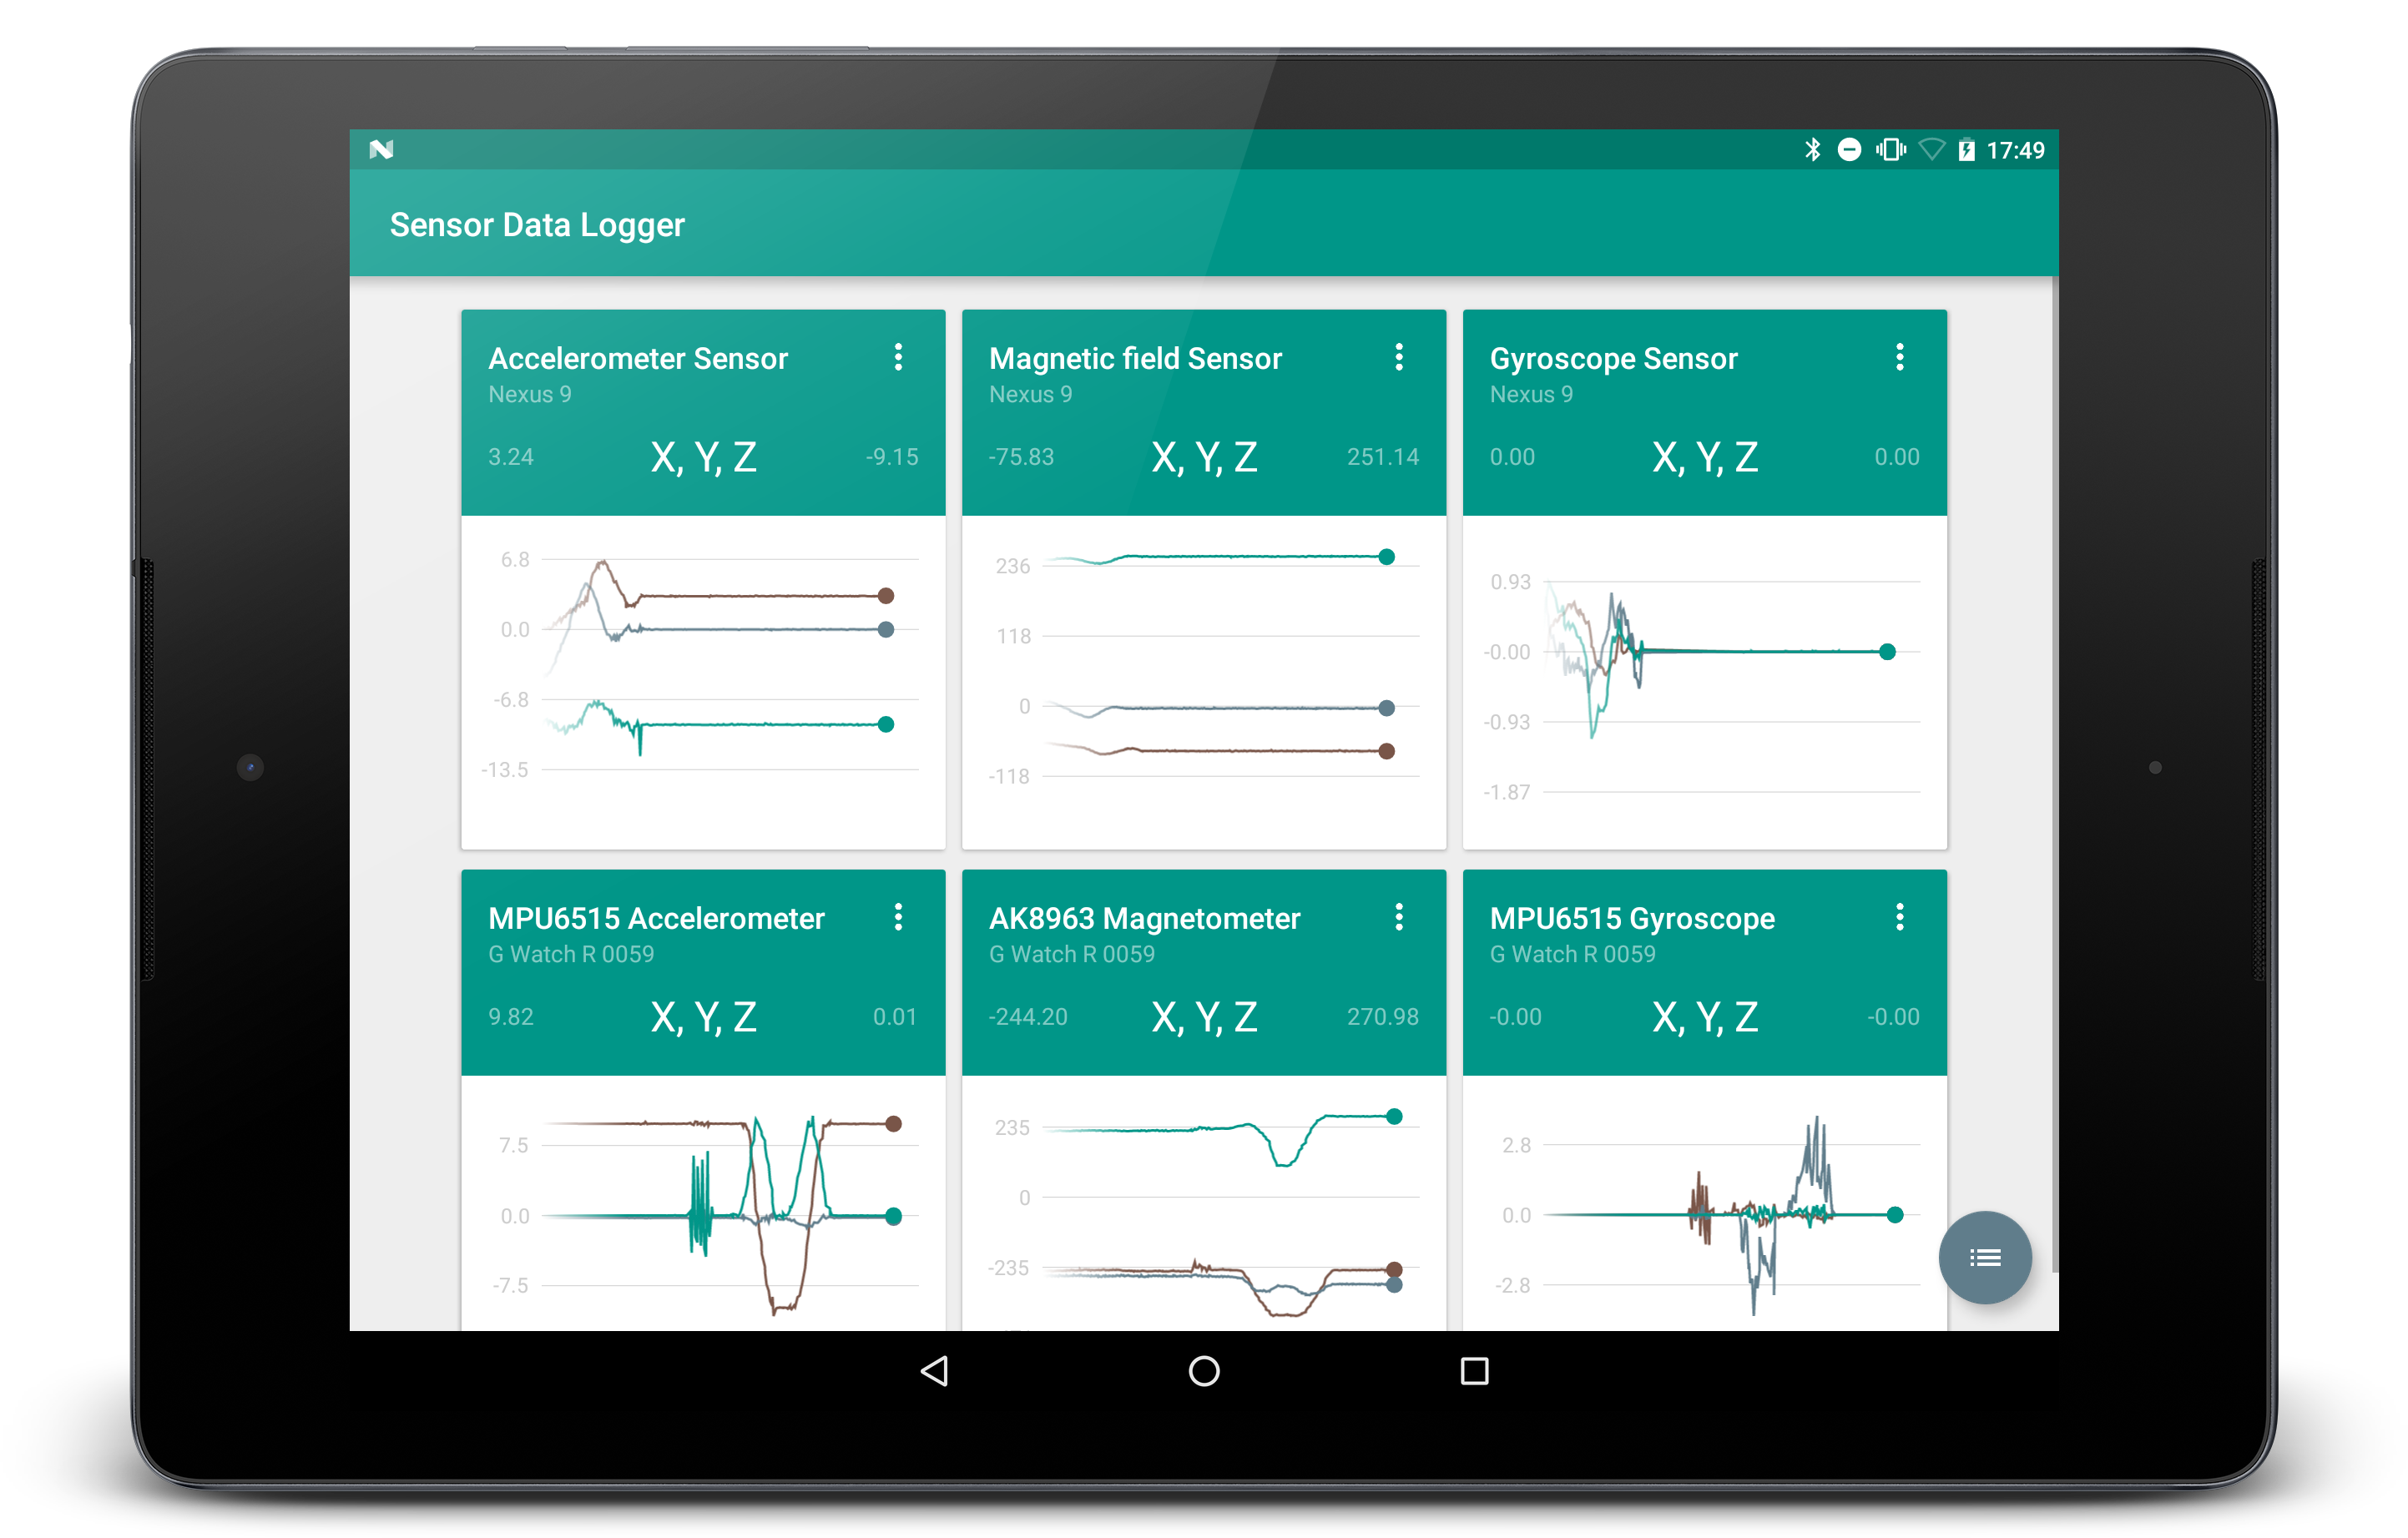
\includegraphics[width=\linewidth]{images/app/charts_landscape_framed.png}
	}
	\caption[Caption for Sensor Data Logger App]{Sensor Data Logger App}
	\label{fig:sensorDataLoggerApp}
\end{figure}

Code samples in the following sections are snippets from this project and can be seen in context in our GitHub repository\footnote{\href{https://github.com/Steppschuh/Sensor-Data-Logger}{https://github.com/Steppschuh/Sensor-Data-Logger}}.

\clearpage

\subsection{Accessing Data}
\label{sec:implementation:accessingdata}

Android provides the |SensorManager|\cite{androiddocs:sensormanager} system service class in order to grant applications access to the device sensors.
The supported sensors can be divided into three categories:

\begin{itemize}[noitemsep]
	\item \textbf{Environmental sensors} (thermometers, barometers and photometers)
	\item \textbf{Motion sensors} (accelerometers, gyroscopes and gravity sensors)
	\item \textbf{Position sensors} (magnetometers and orientation sensors)
\end{itemize}

Not all sensors are hardware components, the so called ``virtual-'' or ``synthetic sensors'' derive their data from one or more hardware-based sensors.
Examples for these virtual sensors are the linear acceleration sensor, which computes its data based on the accelerometer and the gravity sensor.

All sensors can be accessed through the Android sensor framework, which provides classes and interfaces that can be used to figure out which sensors are available on the current device, which capabilities they have and what data they produce.

\subsubsection{Checking Availability}
\label{sec:implementation:checkingavailability}
While most devices have an accelerometer and a magnetometer, only a few have a thermometer.
The availability of sensors can't be guaranteed, it's good practice to check this at runtime:

\begin{lstlisting}[label=getsensormanager]
// get a SensorManager instance
SensorManager sensorManager = (SensorManager) getSystemService(Context.SENSOR_SERVICE);

// get a list of available sensors
List<Sensor> deviceSensors = sensorManager.getSensorList(Sensor.TYPE_ALL);

// check if an accelerometer is available
Sensor accelerometer = sensorManager.getDefaultSensor(Sensor.TYPE_ACCELEROMETER);
if (accelerometer != null) {
	// use accelerometer
} else {
	// perform error handling
}
\end{lstlisting}

If a sensor is available, public methods from the |Sensor|\cite{androiddocs:sensor} class can be used to get detailed information about it.
The name, vendor, version, data range and reporting delay are useful properties, especially because one device can have multiple sensors of the same type.

\subsubsection{Monitoring Data Changes}
\label{sec:implementation:monitoringdatachanges}
In order to get access to the actual data, a |SensorEventListener|\cite{androiddocs:sensoreventlistener} needs to be registered at the |SensorManager| instance. The |SensorEventListener| is an interface which exposes two callback methods:

\begin{lstlisting}[label=registersensoreventlistener]
// create a new SensorEventListener
SensorEventListener listener = new SensorEventListener() {
	@Override
	public void onSensorChanged(SensorEvent event) {
		// sensor reported new data
	}

	@Override
	public void onAccuracyChanged(Sensor sensor, int accuracy) {
		// sensor accuracy changed
	}
};

// specify a reporting delay for the sensor
int delay = SensorManager.SENSOR_DELAY_NORMAL;

// register the listener for the accelerometer
sensorManager.registerListener(listener, accelerometer, delay);
\end{lstlisting}

The |onSensorChanged| method will be called every time the sensor updates its values. The passed |SensorEvent|\cite{androiddocs:sensorevent} holds the sensor, a timestamp, the accuracy and an array of floats containing the actual values.

If the sensor accuracy changes, which often happens when using location sensors, the |onAccuracyChanged| method will be called.
It can be useful to care about these accuracies, the location obtained from the Cell-ID or Wi-Fi might be more accurate than the latest GPS coordinates for example.
In other cases sensors might need a few seconds to calibrate, like the magnetometer.

When registering a |SensorEventListener|, a delay in microseconds is also passed to the |SensorManager|.
It's worth to notice that this value is more like a suggestion, as other applications and the system can alter it.
Because the reporting delay can impact the battery life of the device, some manufacturers will lower the reporting interval when the device is idle or the display is turned off.

\subsubsection{Monitoring Lifecycle Changes}
\label{sec:implementation:monitoringlifecyclechanges}
Once a |SensorEventListener| is registered, the system will keep the requested sensor active and continue to report data, even if the user leaves the application.
Hence, one should always unregister listeners as soon as possible in order to prevent battery drain.

\begin{figure}[H]
	\centering
	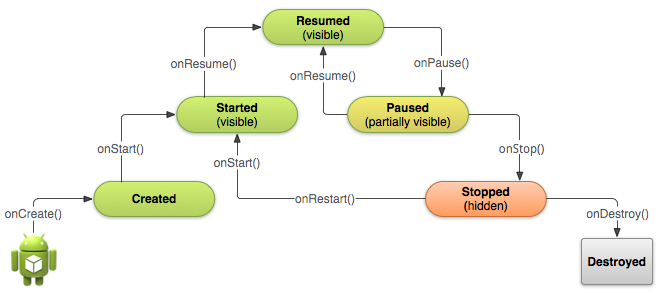
\includegraphics[width=0.85\textwidth]{images/activity_lifecycle.png}
	\caption[Caption for activity_lifecycle]{Activity lifecycle callbacks\footnotemark}
	\label{fig:activityLifecycle}
\end{figure}
\footnotetext{https://developer.android.com/training/basics/activity-lifecycle/starting.html}

We need to have elemental understanding of how the Android |Activity|\cite{androiddocs:activity} lifecycle works, as illustrated in figure \ref{fig:activityLifecycle}.

\clearpage

For a basic implementation, we need to override three |Activity| methods:

\begin{itemize}[noitemsep]
	\item |onCreate()| is called when the |Activity| is first created.
	This is where we will create our view and setup our |SensorManager|.
	\item |onResume()| is called when the activity is at the top of the activity stack and starts interacting with the user.
	We will register our \\|SensorEventListeners| here.
	\item |onPause()| is called when the system is about to start resuming a previous activity.
	We will unregister our |SensorEventListeners| here.
\end{itemize}

The example |Activity| found in Appendix listing \ref{basicactivity} would print accelerometer data to the console while the app is visible to the user.
Keep in mind that it lacks exception handling, as recommended in \ref{sec:implementation:checkingavailability}.

\subsection{Persisting Data}
Once a sensor is reporting data, a new |SensorEvent| will be passed to the callback every few milliseconds.
The |values| float array will contain new data, however the system will not allocate a new object for every update in order to improve performance.
Handling these values without knowing about its object identity might cause confusion, as they will be overwritten with every update.
To prevent this, a new float array can be used to hold the event data:

\begin{lstlisting}[label=arraycopy]
@Override
public void onSensorChanged(SensorEvent event) {
	// create a new float array with the same size
	float[] values = new float[event.values.length];

	// copy data from event values
	System.arraycopy(event.values, 0, values, 0, event.values.length);

	// persist values in some way
	persistValues(values);
}
\end{lstlisting}

\clearpage

For our project, we needed to look back at sensor events from the past few seconds in order to detect patterns and to extract features.
We created some helper classes\cite{sensordatalogger:datapackage} that allowed us to wrap sensor event data in POJOs\footnote{Plain Old Java Objects}, this way they could be persisted in a batch-like structure.

We created a |Data|\cite{sensordatalogger:data} class which can wrap the values of a |SensorEvent|, its source and a timestamp.
This is necessary because the |SensorEvent| holds references to objects that aren't required multiple times and because there's no public constructor available. The |DataBatch|\cite{sensordatalogger:databatch} class holds and manages a list of |Data| objects.
It has a customizable capacity, one can add or remove |Data| and it will automatically remove old |Data| if the capacity has been reached.
It also provides some convenience methods, for example to get |Data| from within a given time range.
The following code would fill up a |DataBatch| with event data for each requested sensor type:

\begin{lstlisting}[label=datahelperclasses]
private Map<Integer, DataBatch> sensorDataBatches = new HashMap<>();

@Override
public void onSensorChanged(SensorEvent event) {
	float[] values = new float[event.values.length];
	System.arraycopy(event.values, 0, values, 0, event.values.length);

	// create a new Data object
	Data data = new Data(values);

	// get a previously initialized DataBatch
	DataBatch dataBatch = getDataBatch(event.sensor.getType());

	// add the new data
	dataBatch.addData(data);
}

public DataBatch getDataBatch(int sensorType) {
	DataBatch dataBatch = sensorDataBatches.get(sensorType);
	if (dataBatch == null) {
		dataBatch = new DataBatch(sensorType);
		sensorDataBatches.put(sensorType, dataBatch);
	}
	return dataBatch;
}
\end{lstlisting}

\subsection{Serializing Data}
\label{sec:implementation:serializingdata}

At some point, we have to convert the persisted data into byte arrays.
We need to serialize objects in order to transfer them to another device or to write it into a file.

The most straightforward solution is using JSON\footnote{JavaScript Object Notation}, which is a common data-interchange format.
It is easy to read for humans and easy to parse for software, which is why we decided to use this format.
Fortunately, POJOs can be directly mapped to JSON name-value pairs.
Existing libraries like gson\footnote{https://github.com/google/gson} or jackson\footnote{https://github.com/FasterXML/jackson} are very well known and provide interfaces that make JSON handling very uncomplicated.

The |DataRequestResponse|\cite{sensordatalogger:datarequestresponse} class for example holds a list of |DataBatches| and is responsible for exchanging sensor data with the connected mobile device.
For convenience, all classes that we transfer implement methods that can be used for JSON serialization and deserialization.

\begin{lstlisting}[label=serialization]
@JsonIgnore
public String toJson() {
	String jsonData = null;
	try {
		ObjectMapper mapper = new ObjectMapper();
		mapper.enable(SerializationFeature.INDENT_OUTPUT);
		mapper.disable(SerializationFeature.FAIL_ON_EMPTY_BEANS);
		jsonData = mapper.writeValueAsString(this);
	} catch (Exception ex) {
		ex.printStackTrace();
	}
	return jsonData;
}
\end{lstlisting}

\clearpage

\begin{lstlisting}[label=deserialization]
public static DataRequestResponse fromJson(String json) {
	DataRequestResponse dataRequestResponse = null;
	try {
		ObjectMapper mapper = new ObjectMapper();
		mapper.disable(SerializationFeature.FAIL_ON_EMPTY_BEANS);
		dataRequestResponse = mapper.readValue(json, DataRequestResponse.class);
	} catch (Exception ex) {
		ex.printStackTrace();
	}
	return dataRequestResponse;
}
\end{lstlisting}

This code block is part of the |DataRequestResponse| class.
The |toJson()| method writes the current object state into a JSON string, while |fromJson(String json)| creates a new |DataRequestResponse| object from a given JSON string.
The JSON string can be converted to a byte array, which can be transferred as described in section \ref{sec:implementation:transferringdata}.
It is crucial that the same character encoding is used, we stick with UTF-8.

\clearpage

\subsection{Transferring Data}
\label{sec:implementation:transferringdata}
Actually using the sensor event data requires transferring it to a device with sufficient processing power.

\subsubsection{General Approach}
In a world where the IoT\footnote{Internet of Things} is a big topic, data is usually uploaded to the cloud and processed on powerful servers.
Although one could do that from a mobile device, this approach would produce a huge amount of traffic and ultimately lead to privacy concerns.

\begin{figure}[H]
	\centering
	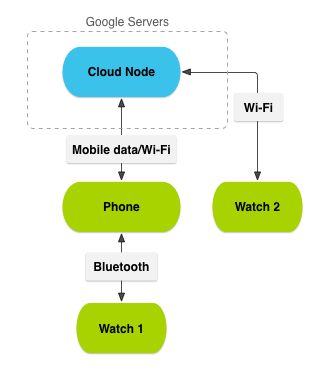
\includegraphics[width=0.5\textwidth]{images/wear_cloud_node.png}
	\caption[Caption for wear_cloud_node]{Sample network with mobile and wearable nodes\footnotemark}
	\label{fig:nodeNetwork}
\end{figure}
\footnotetext{https://developer.android.com/training/wearables/data-layer/}

The setup that this work is about could be seen as a peer to peer network between a mobile device and multiple wearables.
Because the devices are connected with each other, there's no need to detour data through the internet.

\clearpage

By default, wearables are connected via Bluetooth with a mobile device.
On the Android platform, this connection can be accessed through the |WearableApi|\cite{androiddocs:wearable}.

\subsubsection{The Wearable Data Layer}

The Data Layer API is part of of the Google Play Services.
It contains the only APIs that should be used to set up a communication channel between a mobile device and wearable devices. 
Custom, low-level socket implementations are not recommended.

As shown in figure \ref{fig:nodeNetwork}, the Data Layer API can handle multiple nodes at once.
We are particularly interested in the Bluetooth channel, but we don't have to care about the connection because this is handled by the Play Services for us.
The API can be reached using an instance of the |GoogleApiClient|\cite{androiddocs:googleapiclient}.
Because some Play Services may not be available on every device, the |GoogleApiClient| needs to be setup first:

\begin{lstlisting}[label=googleapiclient]
GoogleApiClient googleApiClient = new GoogleApiClient.Builder(context)
		.addConnectionCallbacks(new ConnectionCallbacks() {
			@Override
			public void onConnected(Bundle connectionHint) {
				// start using the Data Layer API
			}
			@Override
			public void onConnectionSuspended(int cause) {
				// something interrupted the connection
			}
		})
		.addOnConnectionFailedListener(new OnConnectionFailedListener() {
			@Override
			public void onConnectionFailed(ConnectionResult result) {
				// API might not be available
			}
		})
		.addApi(Wearable.API)
		.build();
\end{lstlisting}

\clearpage

This code block would initialize a |GoogleApiClient| instance.
However, \\|addApi(Wearable.API)| would cause a call to |onConnectionFailed| if the device it runs on doesn't have the Android Wear app\footnote{https://play.google.com/store/apps/details?id=com.google.android.wearable.app} installed.
This app is required because it handles the connection and synchronization of wearables.
For more graceful error handling, |addApiIfAvailable(Wearable.API)| might be the more appropriate solution.

\subsubsection{The Message API}

There are multiple ways of exchanging data between nodes using the Data Layer API.
While the |DataApi|\cite{androiddocs:dataapi} can be used to synchronize larger binary blobs (|Assets|\cite{androiddocs:asset}) across the wearable network, the |MessageApi|\cite{androiddocs:messageapi} is more suitable for exchanging smaller amounts of data.
A message consists of the following items:
\begin{itemize}[noitemsep]
	\item \textbf{Path}:
	A string that uniquely identifies the message action. 
	\item \textbf{Payload}:
	An optional byte array.
\end{itemize}
Payloads are not required by default because messages are a one-way communication mechanism, often used to only trigger RPCs\footnote{Remote procedure calls}. We use this to pass a serialized |DataRequest|\cite{sensordatalogger:datarequest} or |DataRequestResponse|\cite{sensordatalogger:datarequestresponse}.

\clearpage

\subsubsection{Sending Messages}
\label{sec:implementation:transferringdata:send}

In order to send a message to a connected wearable, the |Node|\cite{androiddocs:node} representation of that device is required.
We can use the |NodeApi|\cite{androiddocs:nodeapi} to query connected nodes:

\begin{lstlisting}[label=nodes]
// a list that holds available nodes
private List<Node> nearbyNodes;

private void updateNearbyNodes() {
	Wearable.NodeApi.getConnectedNodes(googleApiClient)
			.setResultCallback(new ResultCallback<NodeApi.GetConnectedNodesResult>() {
				@Override
				public void onResult(NodeApi.GetConnectedNodesResult nodes) {
					nearbyNodes = new ArrayList<Node>();

					// add all nearby nodes to the list
					for (Node node: nodes.getNodes()) {
						if (node.isNearby()) {
							nearbyNodes.add(node);
						}
					}
				}
			});
}
\end{lstlisting}

\clearpage

The |nearbyNodes| list now contains all currently connected wearables.
We can get a display name and an id for each node, which we need to select our message target.
For simplicity, the following code block sends a message to all nearby nodes:

\begin{lstlisting}[label=sendmessage]
private void startRequestingSensorData() {
	// send a request message to all nodes
	sendMessageToNearbyNodes("/start_requesting_sensor_data", null);
}

private void sendMessageToNearbyNodes(String path, byte[] payload) {
	for (Node node: nearbyNodes) {
		sendMessageToNode(node.getId(), path, payload);
	}
}

private void sendMessageToNode(String nodeId, String path, byte[] payload) {
	Wearable.MessageApi.sendMessage(googleApiClient, nodeId, path, payload)
			.setResultCallback(new ResultCallback() {
				@Override
				public void onResult(SendMessageResult sendMessageResult) {
					if (!sendMessageResult.getStatus().isSuccess()) {
						// perform exception handling
					}
				}
			});
}
\end{lstlisting}

Note that we can pass |null| as a payload if no data is required.
Instead of null, a serialized |DataRequest| object could be passed.
The receiving nodes could deserialize it to find out which sensors are requested or at which interval they should report updates.

\clearpage

\subsubsection{Receiving Messages}
\label{sec:implementation:transferringdata:receive}

Apps running on the wearables need to implement the |MessageListener|\cite{androiddocs:messagelistener} interface in order to get notified about incoming messages. These listeners have to be registered using the |MessageApi.addListener()| function.

\begin{lstlisting}[label=receivemessage]
@Override
public void onMessageReceived(MessageEvent messageEvent) {
    if (messageEvent.getPath().equals("/start_requesting_sensor_data")) {
        // get the message payload
        byte[] payload = messageEvent.getData();

        // process the request
        startTransferringSensorData();
    }
}
\end{lstlisting}

If no |Activity| context is available, this can also be achieved using the \\|WearableListenerService|\cite{androiddocs:wearablelistenerservice}.
It is capable of receiving events from other nodes, including data changes, messages or connectivity events.

Message paths should be static and final constants defined in a shared module that the mobile and wearable app package have access to. In our implementation, the payload would be a serialized |DataRequest|.

\clearpage